\section{Context switching}
    \begin{tcolorbox}[vert]
        A \important{process} is running instance of a program and are independent of each other. Each process has its own virtual address space and they don't share any system resources. 
    \end{tcolorbox}
    Hundreds of processes can exist on a CPU but only few of them run in parallel at any given time. The OS schedules and switches processes as needed, it gives the illusion of multi-tasking and allows for concurrency (another process runs when one is blocked). For now, P in picture means process not processor.
    \begin{center}
        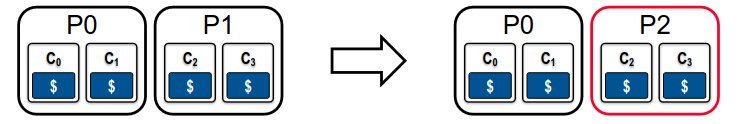
\includegraphics[width=10cm]{images/57.png}
    \end{center}
    \begin{tcolorbox}[vert]
        A single process usually runs multiple \important{threads} at the same time. Threads are independent and can execute various functionality, each has its own program counter, stack and variable values. Unlike processes, threads also share resources: the heap, the code and global data of the process are shared. All threads operate in the same virtual address space.
    \end{tcolorbox}
    \begin{center}
        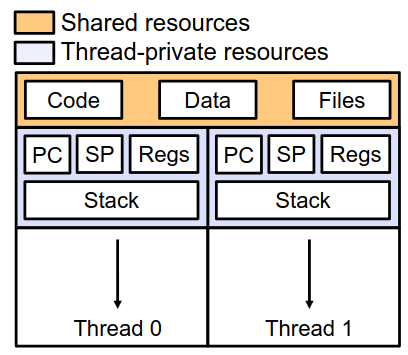
\includegraphics[width=5cm]{images/58.png}
    \end{center}
    We already saw OpenMP, which is simply an easy-to-use abstraction over Pthreads.
    \begin{tcolorbox}[vert]
        \important{POSIX threads (Pthreads)} are general-purpose threads. They are created, scheduled and managed by the kernel, these are also referred to as ``kernel'' threads. They offer fine-grained control over functionality, synchronization and scheduling.
    \end{tcolorbox}
    Many languages offer high-level thread libraries using Pthreads, \lstinline!thread! library in C++ for example, that can be used to build complex multi-threaded programs. Threads can also switch to avoid wasting cycles. 

    For example, in a web server, we can create a new thread every time that we need to handle a new request, so thread 0 can continue to loop and listening for incoming requests. 

    Here is the code example:
    \begin{codeCenter}
    \begin{Ccode}
struct Request {
    ...
};
void handle_request(Request req) {
    ...
}
int main() {
    while (true) {
        auto req = get_next_request();
        if (req) {
            std::thread t(handle_request, *req);
            t.detach();
        } else {
            std::this_thread::sleep_for(std::chrono::milliseconds(50));
        }
    }
    return 0;
}
    \end{Ccode}
    \end{codeCenter}
    \begin{image}{But now imagine we are running the web server on a CPU with four cores, at any given time, only three requests can be handled in parallel.}
        \begin{center}
        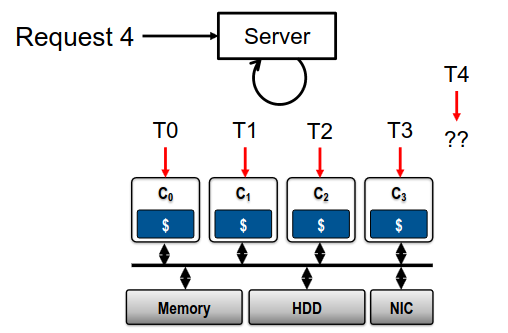
\includegraphics[width=5cm]{images/59.png}
        \end{center}
    \end{image}
    If there is a high rate of incoming requests, the web server will spawn new threads to handle the new requests. These new threads will be locked behind the threads handling the old requests. Then, there is two options: wait for the threads executing the old requests to finish first or context switch threads!
    \begin{tcolorbox}[rouge]
    Let's see that requests can waste cycles. In this code,
    \hypertarget{server}{}
    \begin{codeCenter}
    \begin{Ccode}
struct Request {
    int id, type;
    std::string payload;
};

int hash_arr[N];
void handle_request(Request req) {
    if (req.type == 0) {
        std::ofstream outfile("output.txt", std::ios::app);
        outfile << "Request " << req.id << ": " << req.payload << "\n";
        outfile.close();
    } else if (req.type == 1) {
        hash_arr[req.id] = calc_hash(req.payload);
    }
}
    \end{Ccode}
\end{codeCenter}\hypertarget{type0}{}
    We have two type of request: type 0 write the string into a file, type 1 compute the SHA hash of the string and store it. Writing a single line to a file can take between hundred $\mu s$ to $ms$. So a thread handling a type 0 request is simply IDLE during I/O \textrightarrow \space more than hundred $\mu$s are wasted per line.

    By this time we could serviced around then type 1 request. There is also threads executing type 1 requests that can get blocked behind threads executing type 0 requests that are wasting clock cycles.
    \end{tcolorbox}
    We already saw that parallelism is the ability to execute threads at the same time, to speed up a single task by splitting it among multiple threads. It exploits multiple cores. But what is really concurrency?
    \begin{tcolorbox}[vert]
        \important{Concurrency} is the ability to hide latency among blocked threads, to increase utilization of a core and throughput.
    \end{tcolorbox}
    \begin{center}
        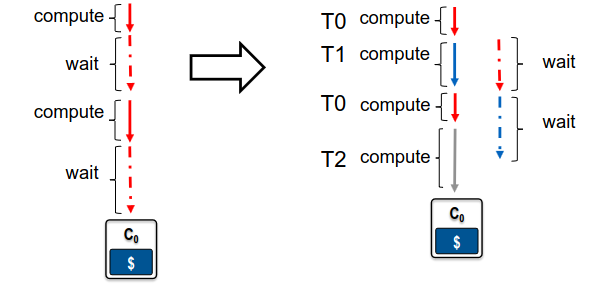
\includegraphics[width=8cm]{images/60.png} 
    \end{center}
    For our code with context switching the kernel would switches the thread with a ``ready'' thread. Once the I/O operation is done, the kernel switches back the waiting thread. 

    The kernel co-ordinates the switch: 
    \begin{enumerate}
        \item It saves the context of the current thread, 
        \item Calls the scheduler algorithm to pick the next thread, 
        \item Restores the context of the next thread.
    \end{enumerate}
    The context save means that we saved the ``state'' of a thread that must be saved before a switch.
    \begin{image}{You need to remember the PC (program counter) of the last executed instruction before the switch, here \lstinline!lw r6, O(r3)!, and also the value of all registers before the switch.}
        \begin{codeCenter}
        \begin{Ccode}
lw r1, 0(r2)
lw r6, 0(r3)

/* Switch to a different thread */
...
/* Resume normal execution */

mul r1, r1, r4
add r6, r1, r6
sw r6, 0(r3)
        \end{Ccode}
        \end{codeCenter}
    \end{image}
    There is no need to save shared resources, only the thread-private ones.

    \begin{tcolorbox}[gris]
    But context switching involves overhead. The explicit one: a syscall means letting the pipeline empty, use the trap table to jump to the syscall code, switch OS. We need also to dump the current thread's context to memory, load the new thread's context and return from syscall, switch back to user. But there is also the implicit overhead: all micro architectural state that is shared (branch tables, TLB, cache hierarchy) is affected while a thread is running.

    Considering all this overhead, context switching is only worth if the time to switch, run and switch back is less that IDLE time, knowing that a single switch between threads in Linux takes ~1-5 $\mu$s. 
    \end{tcolorbox}
    \subsection{User threads}
    Only the kernel has permissions to schedule threads to run on cores. But using the kernel for switching is overkill. So an idea is to separate the two requirements:
    \begin{enumerate}[left=10pt]
        \item Scheduling threads to run on cores - the kernel is needed. 
        \item Switching between threads on the same core - we can actually do this on user threads.
    \end{enumerate}
    \begin{tcolorbox}[violet]
    The creation of a thread is done by the function \lstinline!pthread_create()! that uses a syscall to ask the kernel to create the thread. To create a thread we need to:
    \begin{itemize}[left=10pt, label=\textbullet]
        \item Allocating a data structure to store the context (PC, SP, regs).
        \item Allocating a stack.
        \item Initializing the context.
    \end{itemize}
    \end{tcolorbox}
    So now what if the user created threads instead of the kernel? A user thread library would handle tasks typically done by the kernel: create and manage threads, schedule which thread runs and when, save and restore context during switches.
    \begin{tcolorbox}[vert]
        A thread created entirely in user space is called a \important{user thread}. Thread scheduling happens then at the user level.
    \end{tcolorbox}
    At any given time, only one user thread can run on a core: the user thread either runs to completion or gets blocked. If the user thread gets blocked or completes execution, it need to switch to another user thread. Previously, it was the kernel who detected blocked or completed threads, now it's not possible because the kernel is unaware of these user threads. 
    \begin{tcolorbox}[vert]
        So now the user thread needs to \important{yield} to give back control. It means that it should give up control of the core voluntarily. The user thread library has a scheduler which picks the next user thread to run.
    \end{tcolorbox}
    \begin{tcolorbox}[rouge]
        Here is a pseudocode example of a context switch with  user threads. We first create a new thread by allocating and initializing the context and add the thread to a global queue. Then the function \texttt{yield} saves the context of the current thread, append thread to the queue, gets the next thread from the queue, restores the context of the next thread and resume execution of next thread.
    
    \begin{codeCenter}
    \begin{Ccode}
function create_thread(func):
    thread.context, thread.stack = init()
    thread.function = func
    queue.append(thread)

function yield():
    save_context(current)
    queue.append(current)
    next = queue.pop()
    restore_context(next)
    resume next.function()

function func1():
    ...
    yield()

function func2():
    ...
    yield()
    \end{Ccode}
    \end{codeCenter}
    Then, we done context switching without the kernel!
    \end{tcolorbox}
        So switching is 10-100 times faster than switching between kernel threads because there is no overhead from syscalls and kernel scheduler. We can then make more switch and have a better concurrency.
    \subsection{Coroutines}
    The yielding needs to happen at the same time as the operation that will block our thread. We have to switch before that the part of that block in the function is executed. 
    \begin{tcolorbox}[vert]
        The idea of \important{coroutines} is that the programmer knows when something is going to block the thread so he has functions that can cooperate by pausing and resuming its own function. Cooperative functions or routines are called \important{coroutines}: they are functions that can be paused and resumed. They are implementable through callbacks and language support.
    \end{tcolorbox}
    \begin{tcolorbox}[rouge]
        Let's switch now to retake our \hyperlink{server}{\textit{web server}} code but now in Python:
        \begin{codeCenter}
        \begin{Ccode}
def save_file(req):
    with open('output.txt', 'a') as file:
        file.write(f‘Request {req.id}: {req.payload}‘)
    return
def sha(req):
    hash_arr[req.id] = calc_hash(req.payload)
    return
        \end{Ccode}
        \end{codeCenter}
        The \texttt{save\_file} function execute \hyperlink{type0}{\textit{type 0}} requests and the \texttt{sha} function execute \hyperlink{type0}{\textit{type 1}}. The web server is running on a single core, on the arrival of a request, the corresponding function gets called.
    \end{tcolorbox}
    Implement coroutines requires changing how functions are executed. A normal function call work like this 
    \[\text{Function call } \implies \text{ Function } \implies \text{ Result}\]
    To implement a function defined as a coroutine we have to use \texttt{async}:
    \[\text{\texttt{def save\_file} becomes } \implies \text{\texttt{async def save\_file}}\]
    Then the programmer pauses the function using \texttt{await}: 
    \begin{codeCenter}
    \begin{Ccode}
async def save_file(req):
    with open('output.txt', 'a') as file:
        file.write(f‘Request {req.id}: {req.payload}‘)
    \end{Ccode}
    \end{codeCenter}
    becomes 
    \begin{codeCenter}
    \begin{Ccode}
async def save_file(req):
    with open('output.txt', 'a') as file:
        await file.write(f‘Request {req.id}: {req.payload}‘)
    \end{Ccode}
    \end{codeCenter}
    The \texttt{await} keyword tells Python to pause executing this function until the write is finished and resume on completion of the write. 
    \begin{remark}{Remark}
        Note that \texttt{await} should only be used on other asynchronous functions.
    \end{remark}
    
    \begin{tcolorbox}[gris]
        Calling a coroutine function does not immediately execute it, it returns a coroutine object (an ``awaitable'' in Python) that can be used by the internal Python scheduler that decides when to run and resume execution.
    \end{tcolorbox}
\begin{tikzpicture}[
  box/.style={
    draw, rectangle, minimum width=2.8cm, minimum height=0.75cm,
    align=center, font=\small
  },
  arrow/.style={-{Latex[length=2mm]}, thick},
  code/.style={font=\small\ttfamily},
  >=Latex
]
 
%--- Colonne gauche : flux de contrôle ---
 
% "Function call" label + arrow into Function box
\node[box] (func) {Function};
\node[left=1.5cm of func, align=right, font=\small] (fc) {Function\\ call};
\draw[arrow] (fc.east) -- (func.west);
 
% Callable object
\node[box, below=0.6cm of func] (callable1) {Callable object};
\draw[arrow] (func) -- (callable1);
 
% Scheduler
\node[box, below=0.6cm of callable1] (scheduler1) {Scheduler};
\draw[arrow] (callable1) -- (scheduler1);
 
% Callable object to resume
\node[box, below=0.6cm of scheduler1] (callable2) {Callable object\\ to resume};
\draw[arrow] (scheduler1) -- (callable2);
 
% Bottom row: Scheduler -> Resume -> Result
\node[box, right=0.5cm of callable2] (scheduler2) {Scheduler};
\draw[arrow] (callable2) -- (scheduler2);
 
\node[box, right=0.5cm of scheduler2, minimum width=3.2cm] (resume) {Resume function\\ when unblocked};
\draw[arrow] (scheduler2) -- (resume);
 
\node[box, right=0.5cm of resume] (result) {Result};
\draw[arrow] (resume) -- (result);
 
\end{tikzpicture}
    \begin{remark}{Remark}
        Note that the context is saved in an internal data structure in the user space.
    \end{remark}
    \begin{tcolorbox}[violet]
        
    
    In Python, it is standard to run these functions in a loop on one thread: the internal Python scheduler chooses which function to run, when one function gives up control, another ready function will take control. Here an example of a simple code in Python:
    \begin{codeCenter}
    \begin{Ccode}
import asyncio
import random

async def say_hello(index):
    await asyncio.sleep(random.uniform(0, 2))
    print(f”Hello world, number {index}”)

loop = asyncio.get_event_loop()
loop.run_until_complete(
    asyncio.gather(say_hello(0),say_hello(1),))
    \end{Ccode}
    \end{codeCenter}
    \end{tcolorbox}
    \begin{tcolorbox}[vert]
        The loop that manages all coroutines is called the \important{event loop}, it waits for events (like I/O, timer, messages) and pauses and resumes functions on the completion of events.
    \end{tcolorbox}
    \begin{center}
        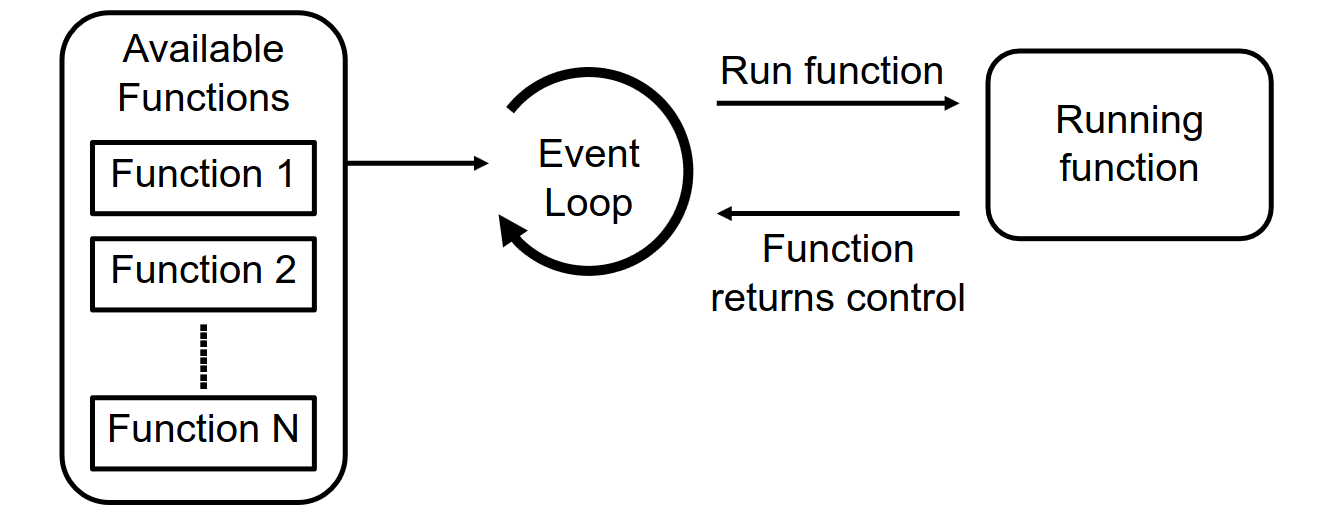
\includegraphics[width=9cm]{images/62.png}
    \end{center}
    Let's now adapt our \hyperlink{server}{\textit{server}}. We have to first modify our function \texttt{save\_file} and \texttt{sha}: we have to turn them asynchronous, we have to make the I/O write function inside asynchronous too and finally we need to wait on the file writing operation. Then our functions look now like this:
    \begin{codeCenter}
    \begin{Ccode}
async def save_file(req):
    async with aiofiles.open('output.txt', 'a') as f:
        await f.write(f‘Request {req.id}: {req.payload}‘)
        
async def sha(req):
    hash_arr[req.id] = calc_hash(req.payload)
    \end{Ccode}
    \end{codeCenter}
    Now, we need to have an event loop to handle incoming requests:
    \begin{codeCenter}
    \begin{Ccode}
async def handle_request(req):
    if req.type == 0:
        await save_file(req)
    elif req.type == 1:
        await sha(req)
        
async def event_loop():
    while True:
        req = await get_next_request()
        if req:
            asyncio.create_task(handle_request(req))
        else:
            await asyncio.sleep(0.05)
    \end{Ccode}
    \end{codeCenter}
